\documentclass{if-beamer}
\usepackage{tikz-cd}
% --------------------------------------------------- %
%                  Presentation info	              %
% --------------------------------------------------- %
\title[Self-interacting Random Walks]{Convergence of self-interacting random walks to Brownian Motion Perturbed at Extrema}
\author[Liu and Wang]{Xiaoyu Liu \and Zhe Wang} % Add the second author here
\institute[Purdue]{Purdue University \and EPFL, Sweden \and \textbf{Mentors: Prof. Jonathon Peterson (Purdue) \and Prof. Thomas Mountford (EPFL)}}


    
\begin{document}

\begin{frame}
  \titlepage
\end{frame}

\section{Random Walks}

\begin{frame}{A random walk in the woods}
    % art.png
    \begin{figure}
        \centering
        \includegraphics[width=1\textwidth]{figures/art.png}
    \end{figure}

\end{frame}

\begin{frame}{Self-Avoiding Walks}

    % two images
    \begin{figure}
        \centering
        \begin{minipage}{0.3\textwidth}
            \centering
            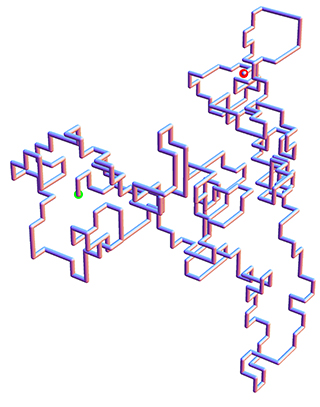
\includegraphics[width=\textwidth]{figures/SAW.jpg}
            \caption{Simulated self-avoiding walk (Math StackOverflow)}
        \end{minipage}
        \hfill
        \begin{minipage}{0.37\textwidth}
            \centering
            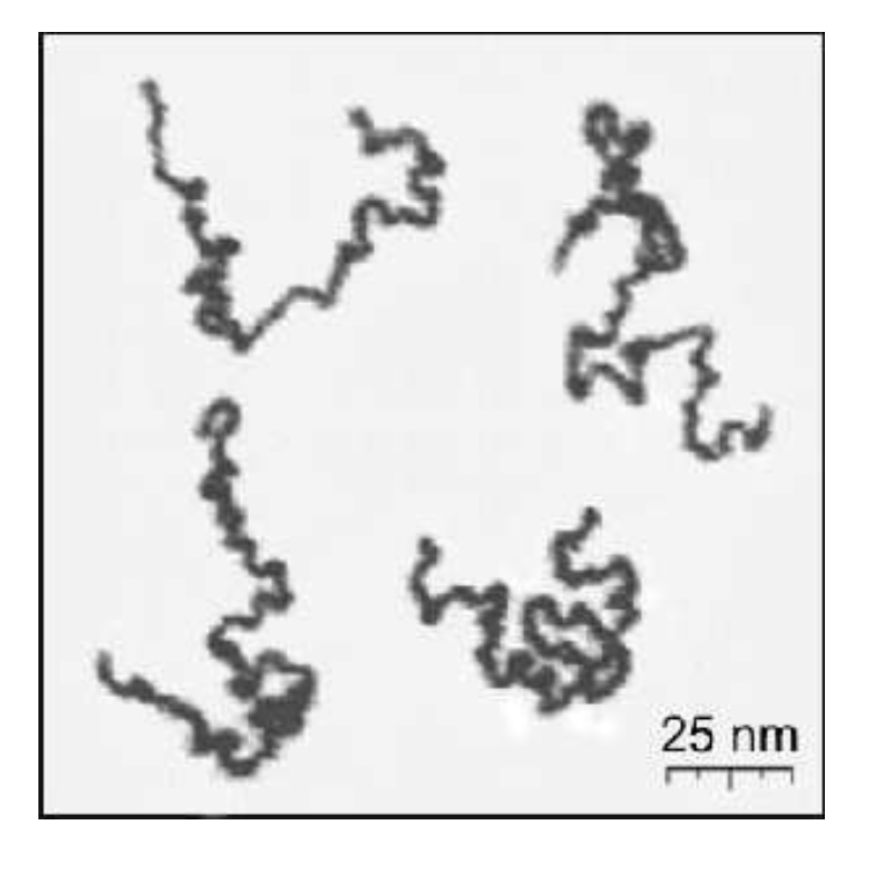
\includegraphics[width=\textwidth]{figures/polymer.png}
            \caption{Polymer chain (Image credit: Roiter and Minko, 2005)}
        \end{minipage}
    \end{figure}

\begin{block}{Why study self-avoiding walks}
    \begin{itemize}
    \item Statistical mechanics
    \item Polymer physics
    \end{itemize}
\end{block}
\end{frame}

\begin{frame}{Self-Interacting Random Walks (Toth, 1996)}

    % two columns
    \begin{columns}
        \begin{column}{0.6\textwidth}
            \begin{block}{Definition}
                \begin{itemize}
                    \item $X_k$ is a random walk on $\mathbb{Z}^1$. At each step, it moves to the left or right.
                    \item <2-> We assign a weight to each edge. 
                    The probability of moving from $x$ to $x+1$ is
                        \begin{align*}
                            &P(X_{k+1} = x+1 | X_k = x) \\
                            &= \frac{wt(x, x+1)}{wt(x-1 ,x) + wt(x, x+1)}
                        \end{align*}
                    \item <3-> The weight $wt(x, x+1)$ is determined by a function $w(n)$ where $n$ is the number of times this edge has been crossed.
                \end{itemize}
            \end{block}
            \begin{exampleblock}<4>{Example}
                $w(n)$ monotone decreasing $\implies$ $X_k$ self-avoiding.
            \end{exampleblock}
        \end{column}
        \begin{column}{0.5\textwidth}
            % figure
            \begin{figure}
                \centering
                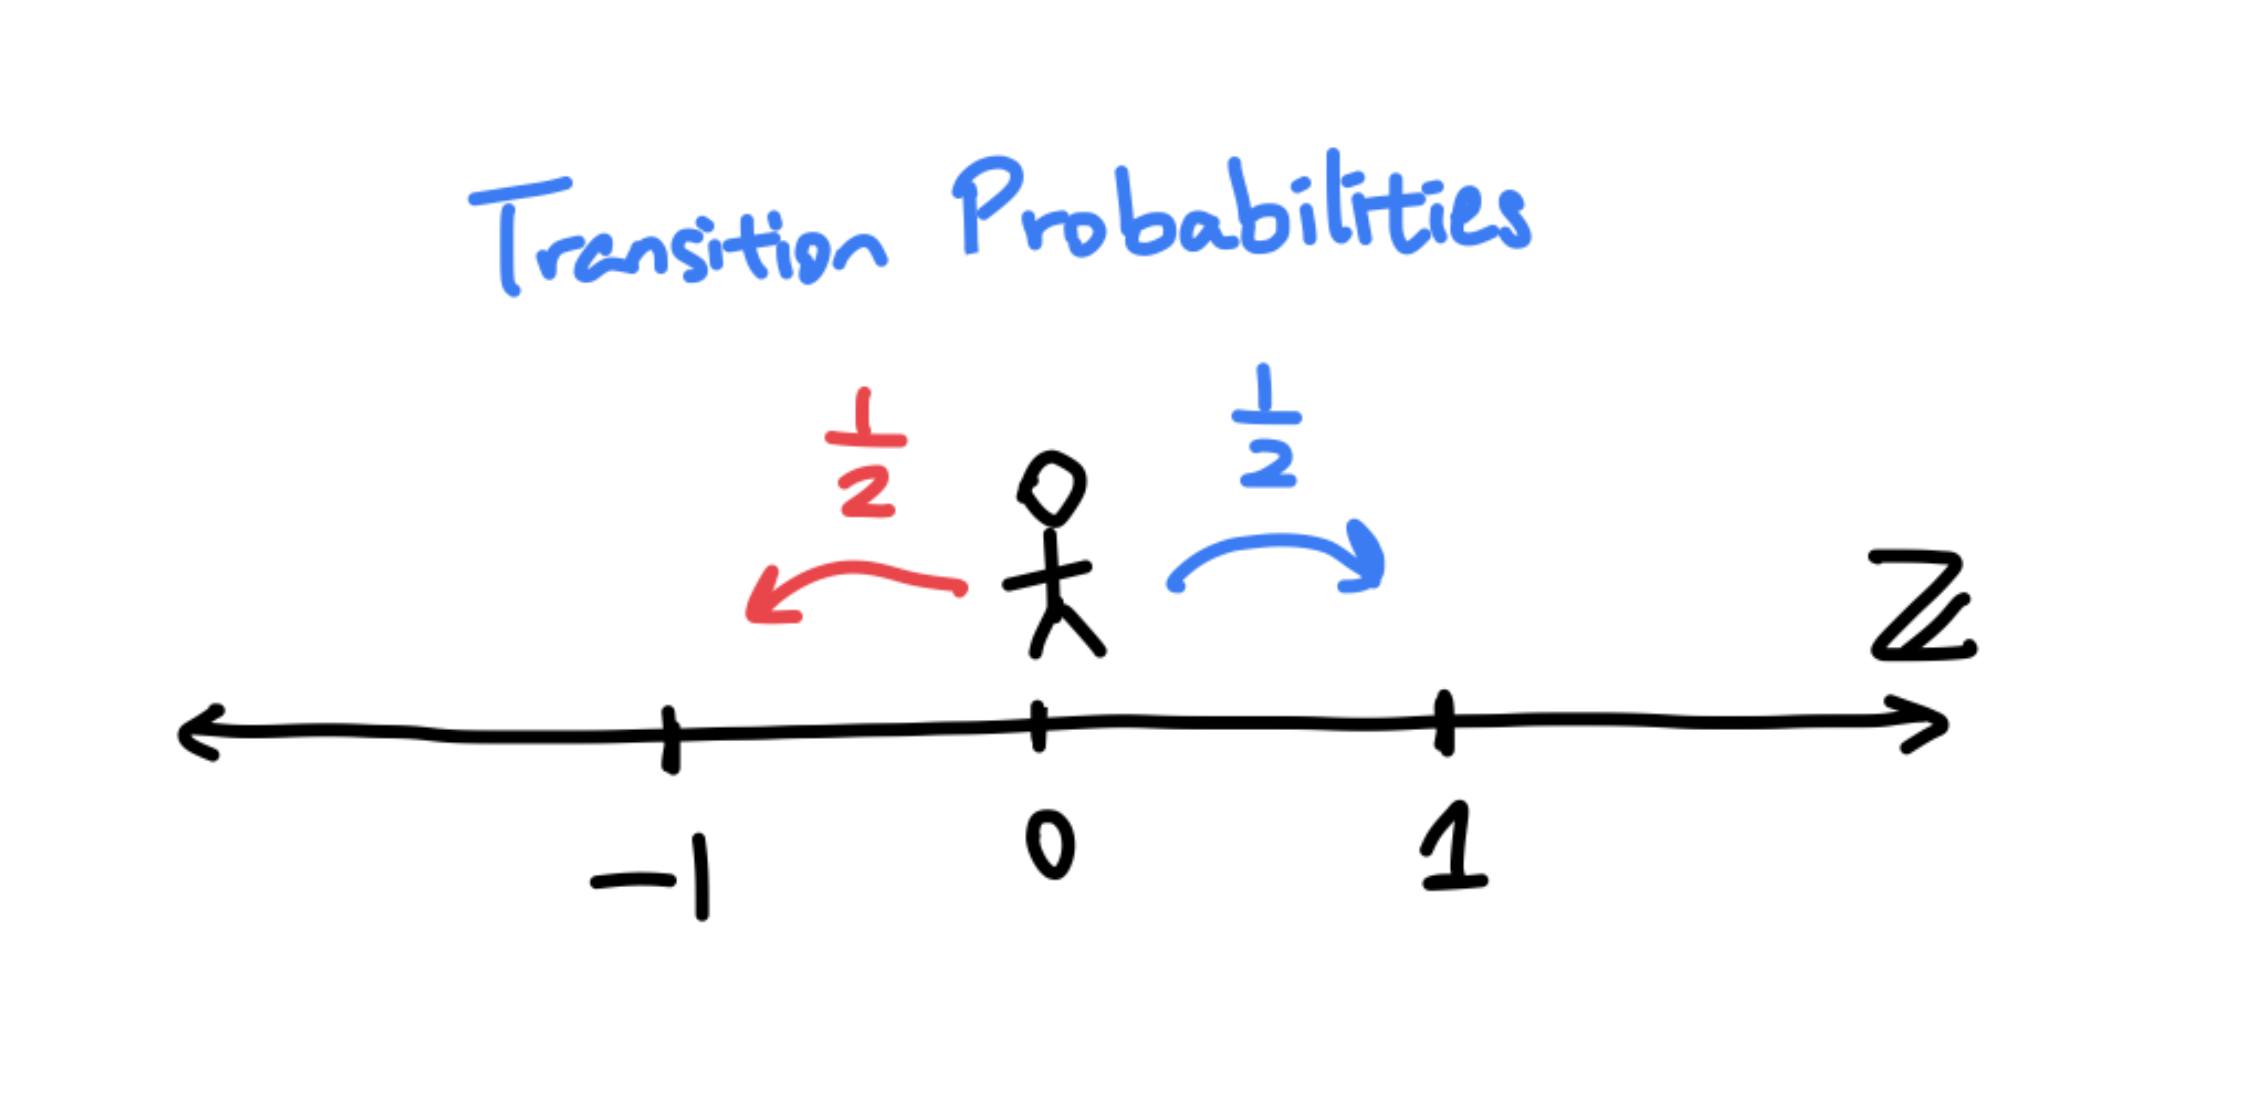
\includegraphics[width=0.7\textwidth]{figures/doodle-def1.png}
                \includegraphics<2->[width=0.7\textwidth]{figures/doodle-def2.png}
                \includegraphics<3->[width=0.7\textwidth]{figures/doodle-def3.png}
            \end{figure}
        \end{column}
    \end{columns}

\end{frame}

\section{Scaling Limit}
\begin{frame}{Scaling behavior in the non-interacting case}
    Consider $w(n) \equiv 1$. This is \textit{simple random walk}.
    
        \begin{minipage}{0.45\textwidth}
            \centering
            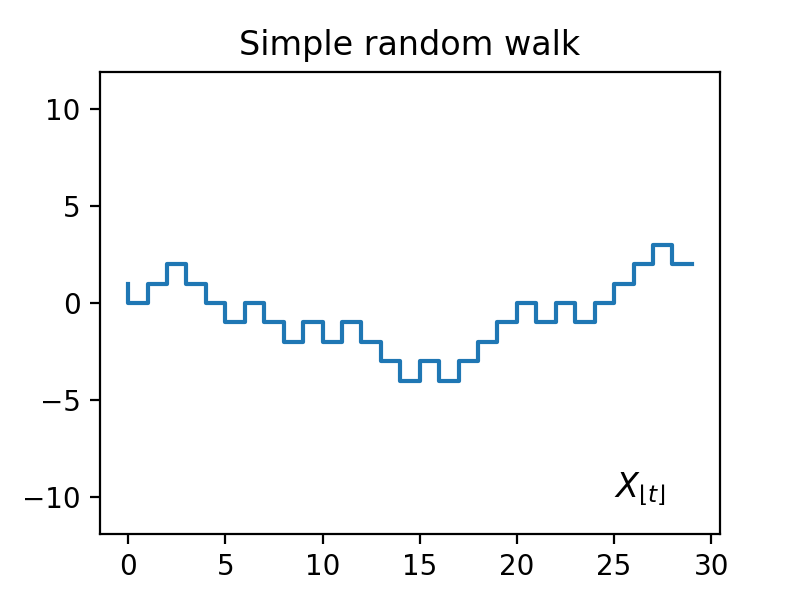
\includegraphics[width=\textwidth]{figures/srw_x1.png}<1>
            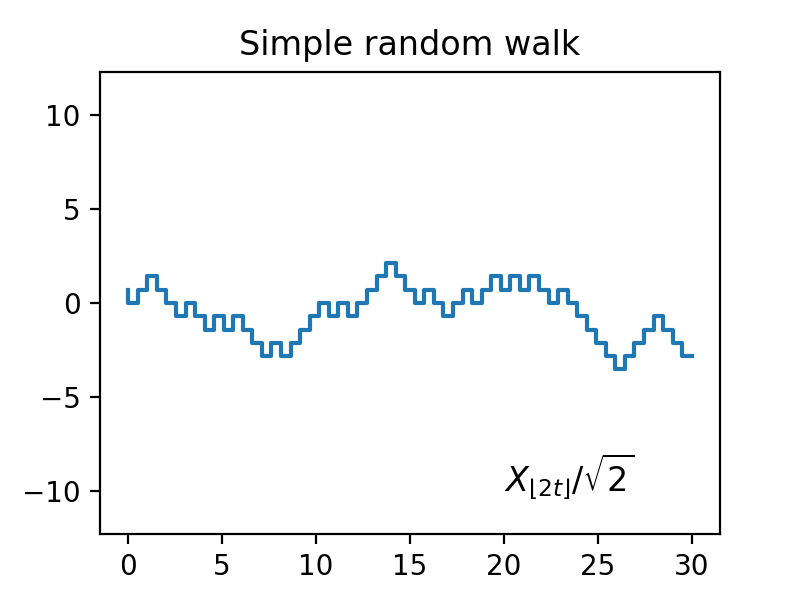
\includegraphics[width=\textwidth]{figures/srw_x2.png}<2>
            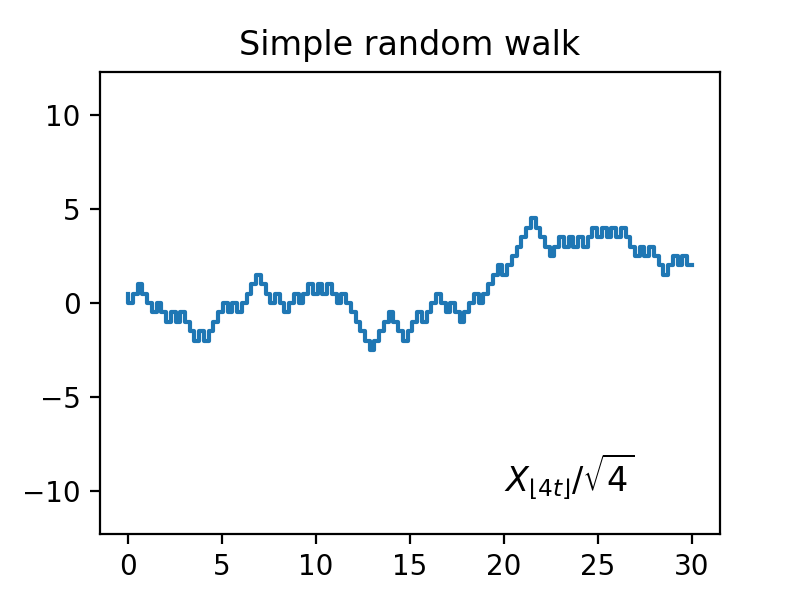
\includegraphics[width=\textwidth]{figures/srw_x3.png}<3>
            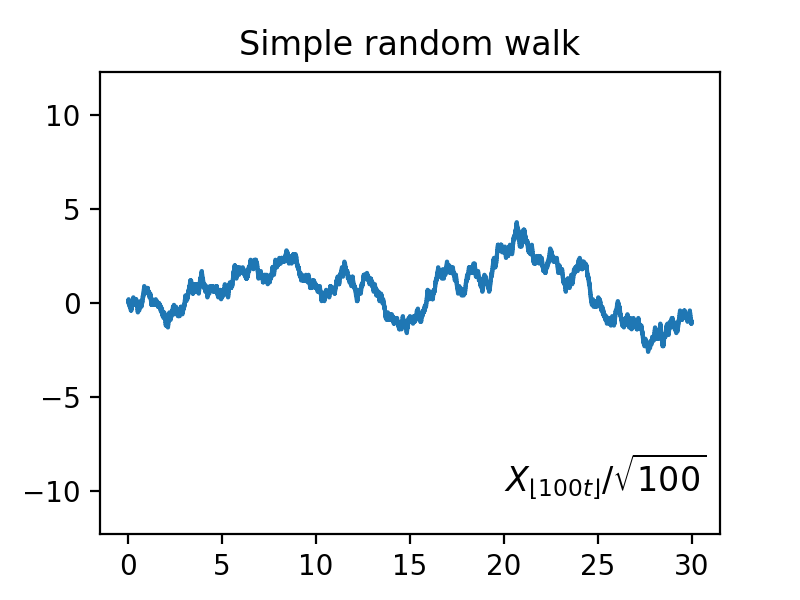
\includegraphics[width=\textwidth]{figures/srw_x4.png}<4->
        \end{minipage}
        \begin{math}
        \uncover<6->{\frac{X_{nt}}{\sqrt{n}} \xrightarrow{n \to \infty} B_t}
        \end{math}
        \begin{minipage}{0.45\textwidth}
            \centering
            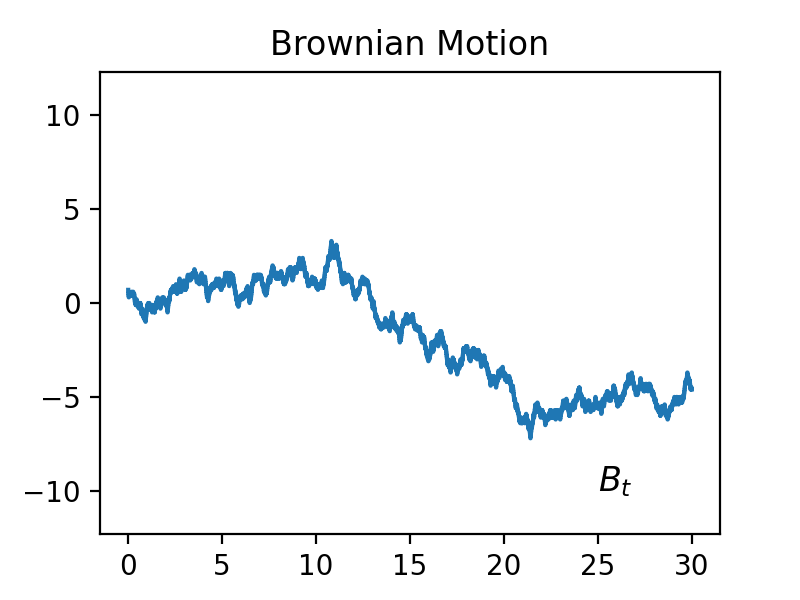
\includegraphics[width=\textwidth]{figures/srw_x5.png}<5->
        \end{minipage}
    % three parallel text blocks
    \begin{block}<7->{Good to know}
        \begin{columns}
            % 3 columns
            \begin{column}{0.3\textwidth}
                \begin{itemize}
                    \item 
                    $ B_t - B_s \sim \mathcal{N}(0, t-s)$
                    \item Markov process
                \end{itemize}
            \end{column}
            \begin{column}{0.3\textwidth}
                \begin{itemize}
                    \item $E(X_{t + s} | X_s) = X_s$
                    \item Martinagle
                \end{itemize}
            \end{column}
            \begin{column}{0.3\textwidth}
                \begin{itemize}
                    \item Visits every point infinitely often
                    \item Recurrent
                \end{itemize}
            \end{column}
        \end{columns}
    \end{block}

    \begin{alertblock}<8->{Question}
        How to understand self-interacting random walks in general?
    \end{alertblock}
\end{frame}

\section{Local Time}

\begin{frame}{Local Time Process}
    \begin{block}{Definition}
        \begin{itemize}
        \item $L(y, T)$, the \textbf{local time} of $X_k$ at site $y$ and time $T$, is the number of times the walk visits $y$ up to time $T$.

        \item $\mathcal{E}(y, T)$, the \textbf{directed edge local time}, is the number of times the walk traverses the edge $(y \to y+1)$ up to time $T$.

        \item $L(\cdot, T)$ and $\mathcal{E}(y, T)$ are random processes on $\mathbb{Z}^1$.
        \end{itemize}
        
    \end{block}

        % figure doodle-blp.png
        \begin{figure}
            \centering
            \includegraphics<1>[width=0.5\textwidth]{figures/doodle-blp.png}
            \includegraphics<2>[width=0.5\textwidth]{figures/doodle-blp2.png}
        \end{figure}

    \pause
    Let $\lambda_{x,m}$ be the time when the walk pays $m$-th visit to $x$.
    
    \begin{alertblock}{Observation}
    On event $\{T = \lambda_{x,m}\}$, the directed edge local time $\mathcal{E}(\cdot, T)$ is a Markov process.

    % It is very similar to a Branching Process.
    \end{alertblock}
\end{frame}

\begin{frame}{Identify scaling limit from local time process}
    The local time process $L(y, \lambda_{x, m})$ is much simpler, and carries scaling information of $X_k$.

    % four figures in two rows,
    \begin{figure}
        \centering
        \begin{minipage}{0.35\textwidth}
            \centering
            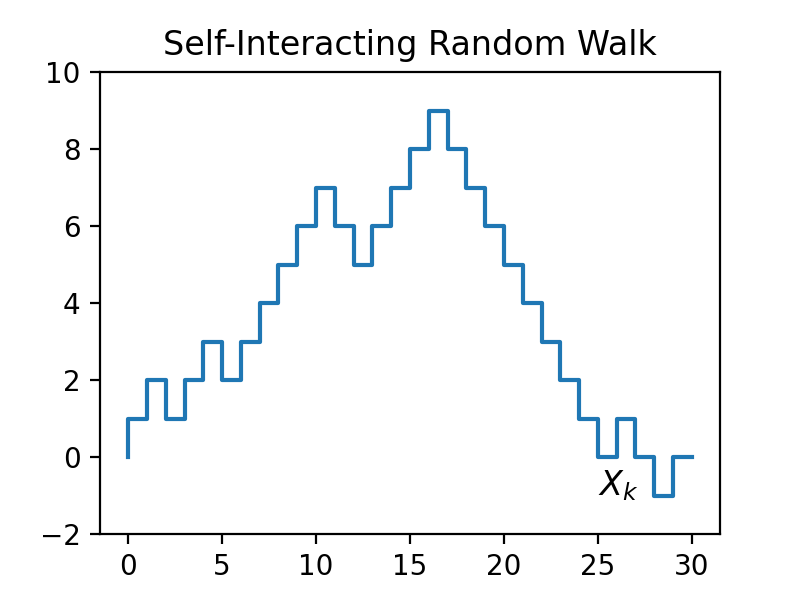
\includegraphics[width=\textwidth]{figures/sirw.png}
            \includegraphics<3->[width=\textwidth]{figures/sirwrescaled.png}
        \end{minipage}
        \begin{minipage}{0.35\textwidth}
            \centering
            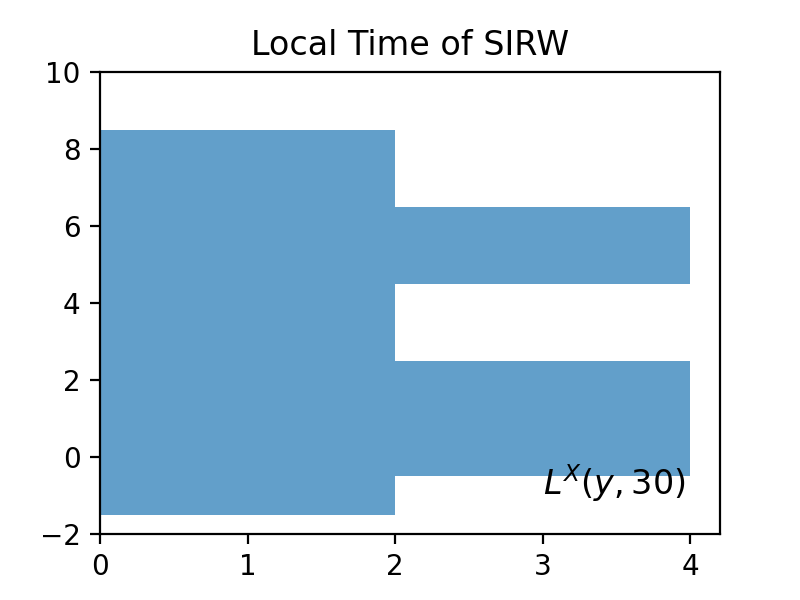
\includegraphics[width=\textwidth]{figures/sirwlocal.png}
            \includegraphics<2->[width=\textwidth]{figures/sirwlocalrescaled.png}
        \end{minipage}
    \end{figure}
\end{frame}
\begin{frame}{Identify scaling limit from local time process}
    \begin{block}{Conjecture (Toth, 1996)}
        If $w(n)$ satisfies certain conditions, then $X_k$ converges after scaling to a Brownian motion perturbed at extrema $W_t$, defined by
        \begin{equation}
            W_t = B_t + \gamma_w (\sup_{s \leq t} W_s + \inf_{s \leq t} W_s)
        \end{equation}
    \end{block}


\end{frame}

\section{Our Results}

\begin{frame}{Our Results}
    \begin{block}{Theorem (Kosygina, Mountford and Peterson, 2023)}
        The convergence $X_k \to W_t$ holds for $w(n)$ satisfying
        \begin{equation*}
            \frac{1}{w(n)}=1+\frac{2^p B}{n^p}+O\left(\frac{1}{n^{1+\kappa}}\right) \quad \text{for some } p\in (\frac{1}{2}, 1], \kappa>0
        .\end{equation*}
    \end{block}
    \pause
    For smaller $p$ there were technical difficulties, resolved in the following theorem.
    \pause
    \begin{block}{Theorem (Liu and Wang, 2024)}
        The previous theorem can be generalized to $p \in (0,1]$.
    \end{block}
    \pause
    \begin{exampleblock}{In search of a general correspondence}
        \begin{minipage}{0.45\textwidth}
% https://quiver.local:8080/#q=WzAsNCxbMCwwLCJYXnsobil9Il0sWzIsMCwiTChYXnsobil9KSJdLFsyLDIsIkwoWSkiXSxbMCwyLCJZIl0sWzAsMV0sWzEsMl0sWzAsMywiIiwyLHsic3R5bGUiOnsiYm9keSI6eyJuYW1lIjoiZGFzaGVkIn19fV0sWzMsMl1d
\[\begin{tikzcd}[ampersand replacement=\&,cramped]
	{X^{(n)}} \&\& {L(X^{(n)})} \\
	\\
	Y \&\& {L(Y)}
	\arrow[from=1-1, to=1-3]
	\arrow[from=1-3, to=3-3]
	\arrow[dashed, from=1-1, to=3-1]
	\arrow[from=3-1, to=3-3]
\end{tikzcd}\]
\end{minipage}
\begin{minipage}{0.45\textwidth}

What precise conditions are necessary to pass from local time convergence to the convergence of the processes themselves?
\end{minipage}
    \end{exampleblock}

        
\end{frame}

\begin{frame}{Main Ideas}
    \begin{itemize}
        \item \emph{Random walks} with \emph{local interactions} are physically and theoretically important.
        \item \emph{Scaling limit} can bring a discrete process on $\mathbb{Z}^1$ to a continuous process on $\mathbb{R}$.
        \item \emph{Local time process} carries information about the scaling limit of the random walk, if it exists.
        \item It would be interesting to understand the general correspondence between the convergence of the local time processes and the convergence of the random walks.
    \end{itemize}
\end{frame}

\begin{frame}
    \begin{center}
        \Huge Questions?
    \end{center}
\vfill
    
\begin{itemize}
\item
    B\'{a}lint T\'{o}th, \emph{Generalized {R}ay-{K}night theory and limit theorems for self-interacting random walks on {${\bf Z}^1$}}, Ann. Probab. \textbf{24} (1996), no.~3, 1324--1367. \MR{1411497}

    \item
    Elena Kosygina, Thomas Mountford, and Jonathon Peterson,  \emph{Convergence and nonconvergence of scaled self-interacting random walks to {B}rownian motion perturbed at extrema}, Ann. Probab. \textbf{51} (2023), no.~5, 1684--1728. \MR{4642221}

    \item
    Patrick Billingsley, \emph{Convergence of probability measures}, second ed., Wiley Series in Probability and Statistics: Probability and Statistics, John Wiley \& Sons, Inc., New York, 1999, A Wiley-Interscience Publication. \MR{1700749}

    \item
    Xiaoyu Liu and Zhe Wang, \emph{Convergence of self-interacting random walks to Brownian Motion perturbed at extrema}, arXiv:2402.11828.

    \end{itemize}
\end{frame}


\end{document}
